\chapter{Erros}
\label{Chap:Erros}

\begin{fullwidth}
{\it
Se precisamos fabricar uma peça de um mecanismo, as tolerâncias nas medidas são em geral muito pequenas, portanto não podemos utilizar equipamentos de medida pouco precisos. Verificaremos que todas as medidas têm um limite de validade dado pela incerteza na medida, sendo que um aumento na precisão de uma medida significa uma diminuição em tal incerteza. Verificaremos quais as origens dos erros e como propagá-los no cálculo de uma medida indireta.
}
\end{fullwidth}

%%%%%%%%%%%%%%%%%%%%%%%%%%%%%%%%%%%%%
\section{Erros de medidas}
%%%%%%%%%%%%%%%%%%%%%%%%%%%%%%%%%%%%%

Se, por exemplo, tomarmos uma trena cujas divisões são em decímetros e a utilizarmos para para medir o diâmetro de um tubo de PVC e com essa informação adquirir uma conexão para o tubo, corremos um grande risco de adquirir uma conexão com um diâmetro inadequado. Claramente estamos usando um instrumento de medida com uma escala inadequada. Nunca é possível se conhecer uma medida com exatidão: Sempre que efetuamos uma medida, a ela estára associada uma incerteza, ou um ``erro''. Determinar esse erro nos permitirá conhecer o limite de utilidade de uma medida. 

Outro fator que dificulta o processo de medida é o fato de que medições sucessivas podem resultar em valores diferentes: se cronometrarmos o tempo de queda de um objeto de uma certa altura com uma precisão razoável, observaremos valores diferentes em cada medida. O tratamento desse tipo de incerteza requer técnicas provenientes da análise estatística, possibilitando a obtenção de um valor mais provável.

Portanto, a determinação do valor de uma medida não é uma tarefa fácil. Além de requerer um método e equipamentos apropriados, precisamos também de uma análise matemática dos resultados para determinar o valor mais adequado. No caso de uma grandeza calculada a partir de outras, precisamos ainda determinar o erro associado, de forma a ter uma ideia de quão confiável é o nosso resultado. Essas tarefas nem sempre são fáceis e dão origem a uma série de métodos que compõe uma \emph{teoria de tratamento de erros e medidas}. No laboratório aplicaremos alguns conceitos descritos a seguir.

%%%%%%%%%%%%%%%%%%%%%%%%%%%%%%%%%%%%%%
\section{Medidas e erros}
%%%%%%%%%%%%%%%%%%%%%%%%%%%%%%%%%%%%%%

Ao efetuarmos uma medição no dia a dia, nos contentamos em atribuir à medida um valor e uma unidade. Expressamos a medida de uma sala, por exemplo, como
\begin{equation}
	\ell = \numprint{4,32}~\textrm{m}.
\end{equation}
Entretanto, associada a toda medida existe uma \emph{incerteza} ou \emph{erro}. Tal erro pode ser composto por três partes: erros sistemáticos, erros de escala e erros aleatórios. Podemos então descrever uma medida mais precisamente ao escrevermos
\begin{equation}
	\ell = (\numprint{4,32} \pm \numprint{0,05})~\textrm{m},
\end{equation}
o que nos diz que além de sabermos que nossa medida é da ordem de \numprint{4,32}~m, ela pode variar de \numprint{0,05}~m para mais ou para menos.

É importante destacarmos que o erro é expresso com somente um algarismo significativo. Uma exceção importante a essa regra é no caso de termos erros cujo primeiro algarismo é 1: nesse caso se admite um erro com dois algarismos significativos. Veremos abaixo os tipos de erro e como calculá-los.


%%%%%%%%%%%%%%%%%%%%%%%%%%%%%%%%%%%%%%%
\subsection{Tipos de erros}
%%%%%%%%%%%%%%%%%%%%%%%%%%%%%%%%%%%%%%%

De uma forma geral, os erros de medida podem ser classificados em três categorias\cite{LivroAmarelo}\cite{LivroEAD}:
\begin{description}
\item[Erros sistemáticos] São erros cuja causa é bem definida e sempre afetam as medidas da mesma maneira. Um exemplo disso são relógios desenvolvidos para usar como padrão de tempo a frequência de oscilação da corrente elétrica de instalações elétricas residenciais. Ocorre, no entanto, que diferentes países adotam frequências diferentes de oscilação da corrente: alguns usam 50~Hz outros 60~Hz (isto é, 50 ou 60 oscilações por segundo). Utilizar um desses relógios em uma região inadequada fará com que ele subestime ou superestime a passagem do tempo. O problema na medida do tempo é sistemático e por isso pode ser corrigido, seja usando um relógio adequado, seja calculando o tempo correto com base no tempo medido.

Apesar do fato de que ---~uma vez conhecido o erro sistemático~--- sua eliminação é relativamente simples, na prática este é um erro bastante difícil de se identificar. O primeiro passo visando garantir que as medidas não tenham erros sistemáticos é calibrar os instrumentos de medida. Tal calibração não pode ser realizada para um único valor, pois o erro pode ser nulo para tal medida e aumentar conforme se aumenta o valor medido. Ainda que essas medidas sejam tomadas, um instrumento pode ter problemas conforme se aumenta a magnitude dos valores a serem medidos, pode não ser exatamente linear para alguma faixa de valores, dentre outros problemas possíveis. No entanto, apesar de todos os cuidados, uma fonte de erro pode passar desapercebida, prejudicando as medidas obtidas.

\item[Erros aleatórios] Um erro aleatório é todo erro que faz variar a medida de maneira imprevisível, porém com igual probabilidade de subestimar ou superestimar o ``valor real'' da medida. Este tipo de incerteza, portanto, se opõe ao erro sistemático, que tente a subestimá-la \emph{ou} superestimá-la. A aleatoriedade da incerteza possibilita que ela seja tratada através de métodos estatísticos, tornando factível a extração de valores de medida precisos através da realização de várias medidas. O fato de a incerteza ser aleatória é algo bom: erros sistemáticos são muito mais difíceis de se eliminar, eliminar e tratar do que simplesmente aumentar o número de medidas e assim diminuir o erro, por mais que isso em geral envolva uma grande quantidade de trabalho para a obtenção dos dados.

Através de cálculos estatísticos, é possível se mostrar que ao se efetuar um grande número de medidas, a melhor estimativa para uma grandeza pode ser extraída através do cálculo da média das medidas. Assim, para um conjunto de medidas $x_1$, $x_2$, \dots, $x_n$, temos que o melhor valor é dado por\footnote{O símbolo $\mean{\;}$ em $\mean{x}$ denota a média da variável $x$.}:
\begin{align}
	\mean{x} &= \frac{x_1 + x_2 + \dots + x_N}{N} \\
		&= \frac{1}{N}\sum_{i=1}^{N} x_i
\end{align}
%
Verificaremos no Capítulo~\ref{Chap:DesvioPadrao} que a incerteza do processo de medição pode ser calculada através dos desvios das medidas em relação ao valor médio. Além disso, verificaremos que a incerteza na média das medidas diminui conforme o número de medidas aumenta, mesmo que cada uma delas tenham a mesma incerteza.

%\item[Erros de escala] Ao realizarmos medidas utilizando um equipamento analógico, verificamos uma série de algarismos com absoluta certeza e estimamos um algarismo adicional. Este algarismo pode acabar sendo subestimado ou superestimado. Temos, portanto, uma situação em que uma parte da medida varia aleatoriamente em torno do ``valor real'' da medida. Podemos tratar esse erro como um erro aleatório e utilizar métodos estatísticos para calcular a incerteza na medida, assumindo que possamos repetir a medição várias vezes. 

%Muitas vezes, no entanto, não podemos. Nesse caso utilizamos o conceito de \emph{erro de escala}. Este tipo de erro é um substituto \comment{Não sei se o erro de escala é um substituto ou é simplesmente algo que somamos. A variação aleatória pode ser real (influência do ar, por ex.) à qual se deve somar o erro inerente à leitura do aparelho. Ver isso.} simplificado dos resultados para a incerteza que seriam obtidos através do método estatístico, usado para tratar erros aleatórios. Através dele, conseguimos uma estimativa razoável do erro que um equipamento possui simplesmente avaliando o tamanho da menor divisão da escala. Se calcularmos o erro dessa forma ou utilizarmos o método estatístico, obteremos valores parecidos. A vantagem de utilizar o erro de escala é sua simplicidade (se comparado ao estatístico) e o fato de que podemos utilizá-lo mesmo em um número pequeno de medidas.

%Em algumas situações, no entanto, o erro de escala pode subestimar o erro real. Um exemplo disso é o uso de cronômetros manuais nos quais a menor divisão da escala está em centésimos de segundo. Se utilizarmos o erro de escala, teremos um erro de um centésimo de segundo na medida. No entanto, o tempo de reação do usuário do cronômetro é maior do que o erro de escala, o que certamente implicará em um erro muito maior, provavelmente da ordem de décimos de segundo. Este caso ilustra a maior limitação desse método. De qualquer forma, devido a sua simplicidade, este será o método que utilizaremos  em nossos procedimentos de laboratório. Veremos suas propriedades em mais detalhes na próxima seção.
%\end{description}

\item[Erros de escala] Ao realizarmos medidas utilizando um equipamento analógico, verificamos uma série de algarismos com absoluta certeza e estimamos um algarismo adicional. Este algarismo pode acabar sendo subestimado ou superestimado durante a leitura da escala do instrumento. Temos, portanto, uma fonte adicional de erros. 
%A largura do intervalo em torno da melhor estimativa pode depender da distância entre as as marcas da escala, sendo menor se a distância for grande, porém se a distância é pequena, adotamos um erro equivalente à metade de tal distância. 

De maneira similar, em equipamentos digitais não sabemos qual seria o próximo digito caso utilizássemos um equipamento com maior precisão e não sabemos se o equipamento simplesmente descarta os demais dígitos ou os utiliza para realizar arredondamentos. Assim a melhor estimativa da medidao pode estar contida em um intervalo acima ou abaixo do valor apresentado pelo instrumento de medida. Portanto também temos fontes de incerteza relacionadas à medida no caso de um equipamento digital.

Em ambos os casos as incertezas estão ligadas à leitura das medidas e dependem das escalas utilizadas nos instrumentos de medida, dando origem ao que denominamos como \emph{erros de escala}. Esse tipo de erro é o mais relevante para os experimentos realizados nos laboratórios didáticos, e o veremos em mais detalhes na próxima seção.
\end{description}

O erro total de uma medida é então composto pelos três erros descritos acima. Em uma situação qualquer, um deles pode ser muito maior que os demais, determinando o valor do erro. Um exemplo disso é o uso de cronômetros manuais nos quais a menor divisão da escala está em centésimos de segundo. Verificando o erro de escala, teremos um erro de um centésimo de segundo na medida\footnote{Veremos adiante como determinar o erro de escala.}. No entanto, o tempo de reação do usuário do cronômetro é maior do que o erro de escala, levando a um erro aleatório da ordem de \np[s]{0,2}. Nesse caso o erro total é dado por \np[s]{0,21}, porém como utilizamos somente um algarismo significativo para denotar o erro, temos um erro de \np[s]{0,2}, que é o próprio erro aleatório ---~isto é, o erro aleatório é dominante~---.

Quando temos um tipo de erro que é muito maior que os outros, precisamos considerar somente o erro dominante, descartando os demais. Em geral é isso o que acontece com medidas estáticas, como as realizadas por um paquímetro ou por uma régua: nesse caso o erro dominante é o de escala, enquanto o aleatório é desprezível. Como esse é o caso da maioria das medidas realizadas nas experiências de laboratório didático, focaremos nossa atenção predominantemente neste tipo de erro. Devido às dificuldades em tratar os erros sistemáticos, consideraremos que os aparelhos utilizados estejam devidamente calibrados e que não existe nenhum erro sistemático relevante.


%%%%%%%%%%%%%%%%%%%%%%%%%%%%%%%%%%%%%%%%%%%%%%
\section{Erros de escala em uma medida direta}
%%%%%%%%%%%%%%%%%%%%%%%%%%%%%%%%%%%%%%%%%%%%%%

Podemos dividir a questão do erro de escala de uma medida direta em dois casos, conforme o tipo de equipamento que estamos utilizando:
\begin{description}
	\item[Equipamentos analógicos:] Se utilizarmos um equipamento analógico ---~como uma régua milimetrada, por exemplo~--- podemos verificar medidas menores que \np[mm]{1} se estimarmos valores entre uma casa de milímetros e outra. Podemos dizer que o erro associado deve ser claramente menor que \np[mm]{1}, pois ao realizar uma medida de ---~por exemplo~--- $\np[cm]{13,41}$, um erro de \np[mm]{1} poderia levar essa medida ao valores extremos $\ell - \delta\ell = \np[cm]{13,31}$ e $\ell+\delta\ell = \np[cm]{13,51}$: Claramente há um exagero, afinal tais medidas estariam muito próximas das marcas de \np[cm]{13,3} e \np[cm]{13,5} que conseguimos distinguir perfeitamente em uma régua. Um valor menor para o erro parece uma melhor ideia. Se tomarmos um valor para o erro de \np[mm]{0,5}, os valores extremos de $\ell$ se tornariam mais razoáveis, pois não poderíamos afirmar com tanta certeza de que não se tratam de valores claramente distinguíveis em uma medida: $\ell - \delta\ell = \np[cm]{13,36}$ e $\ell+\delta\ell = \np[cm]{13,46}$.

\begin{marginfigure}
	\includegraphics[width=\textwidth]{Ilustrations/AmperimetroAnalogEspelho.png}
	\caption{Para eliminar erros de leitura devidos à paralaxe, muitos equipamentos utilizam um espelho atrás do ponteiro (região curva abaixo da escala): quando a imagem do ponteiro no espelho está atrás do próprio ponteiro, temos certeza de que estamos vendo o ponteiro exatamente de frente, eliminando este tipo de erro.}
\end{marginfigure}

	Um erro pequeno pode ser cometido na própria leitura dos valores devido à paralaxe (deslocamento aparente entre dois objetos localizados a distâncias diferentes do observador quando este se move). Isso é bastante notável em equipamentos analógicos em que a medida é mostrada por um ponteiro, pois quando o observador se desloca uma pequena distância para um lado ou outro, a posição aparente do ponteiro muda. Para evitar o erro de paralaxe, a medida deve ser feita de forma que o ponteiro seja observado diretamente de frente. Alguns aparelhos têm uma região espelhada atrás do ponteiro para eliminar esse tipo de erro, sendo que a leitura correta é feita quando a imagem do ponteiro fica escondida atrás dele.
	
	Em alguns equipamentos, a menor divisão da escala ---~o que denominamos como \emph{resolução} do equipamento~--- pode ser muito grande. Nesse caso, temos mais facilidade em avaliar o algarismo estimado. Podemos então reduzir o valor do erro para \nicefrac{1}{3} ou \nicefrac{1}{4} da medida. No entanto isso não é muito comum, pois em geral os fabricantes dos equipamentos optam por divisões pequenas com o intuito de possibilitar a realização de medidas precisas. Nos equipamentos que utilizaremos no laboratório didático, as divisões são em geral pequenas e por isso adotaremos sempre que o erro é equivalente à metade da menor divisão da escala.

\begin{marginfigure}
    \centering
    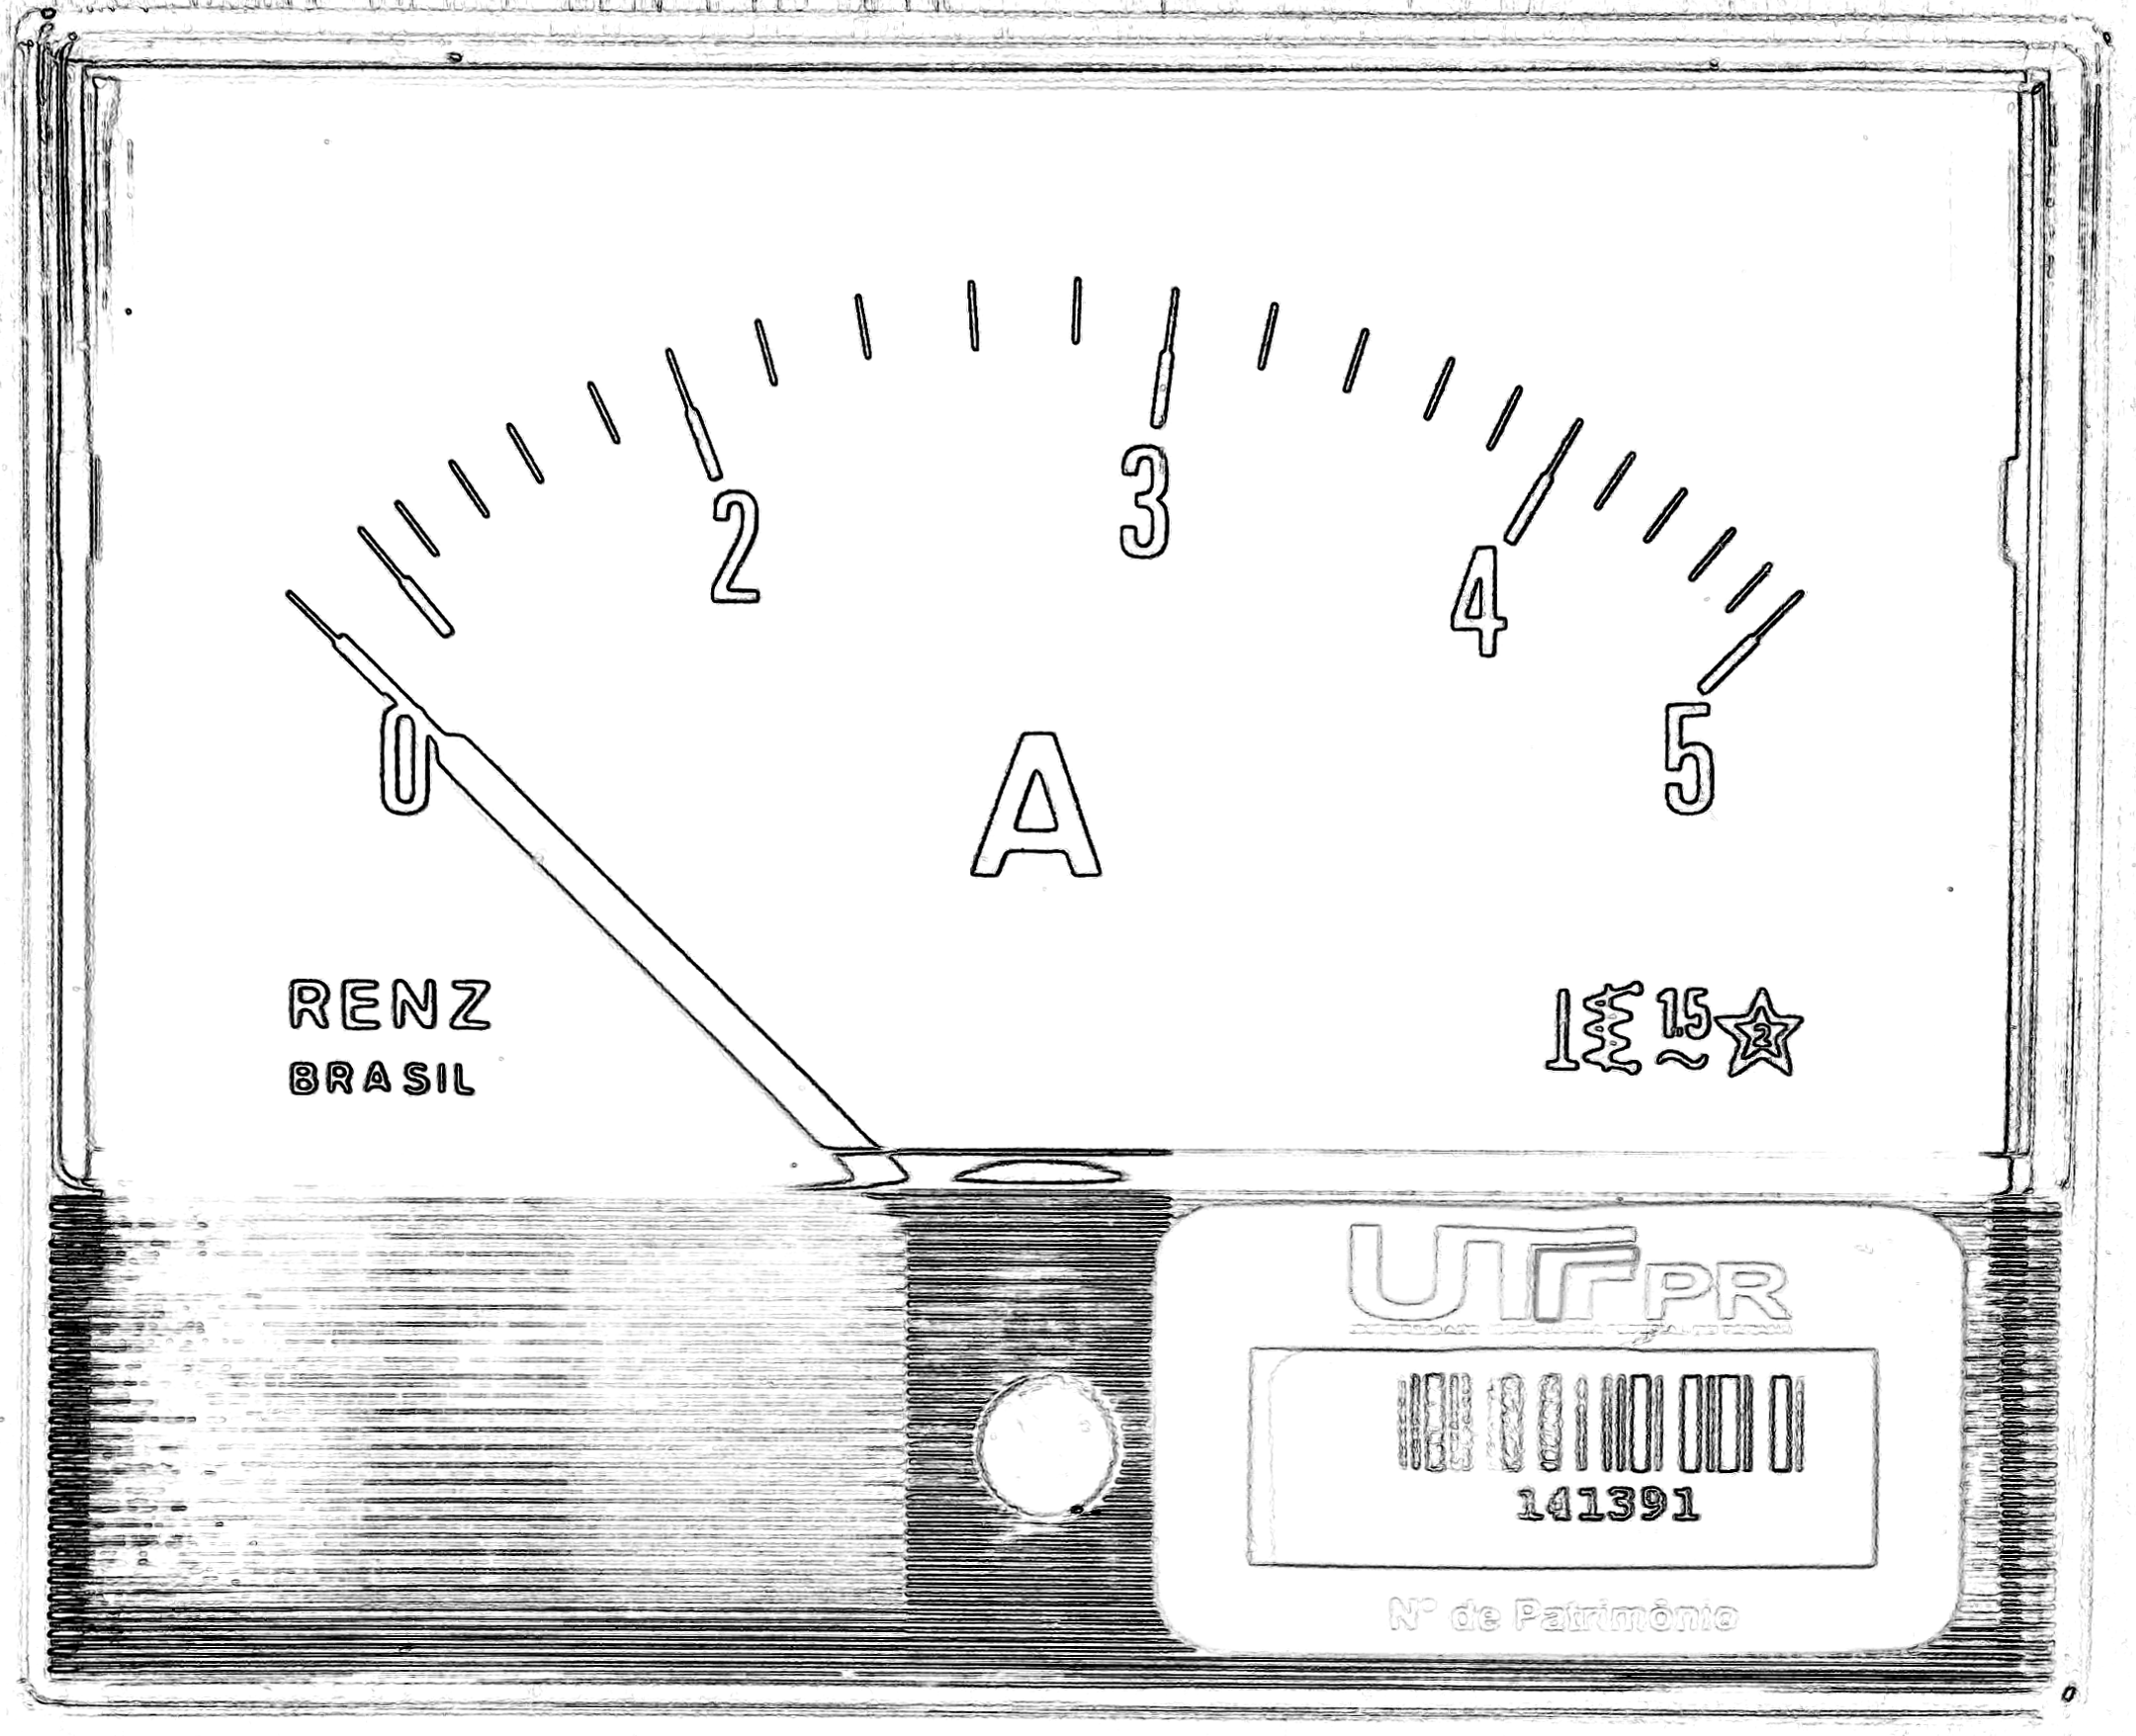
\includegraphics[width=\linewidth]{Ilustrations/EscalaGrandeDiv.png}
    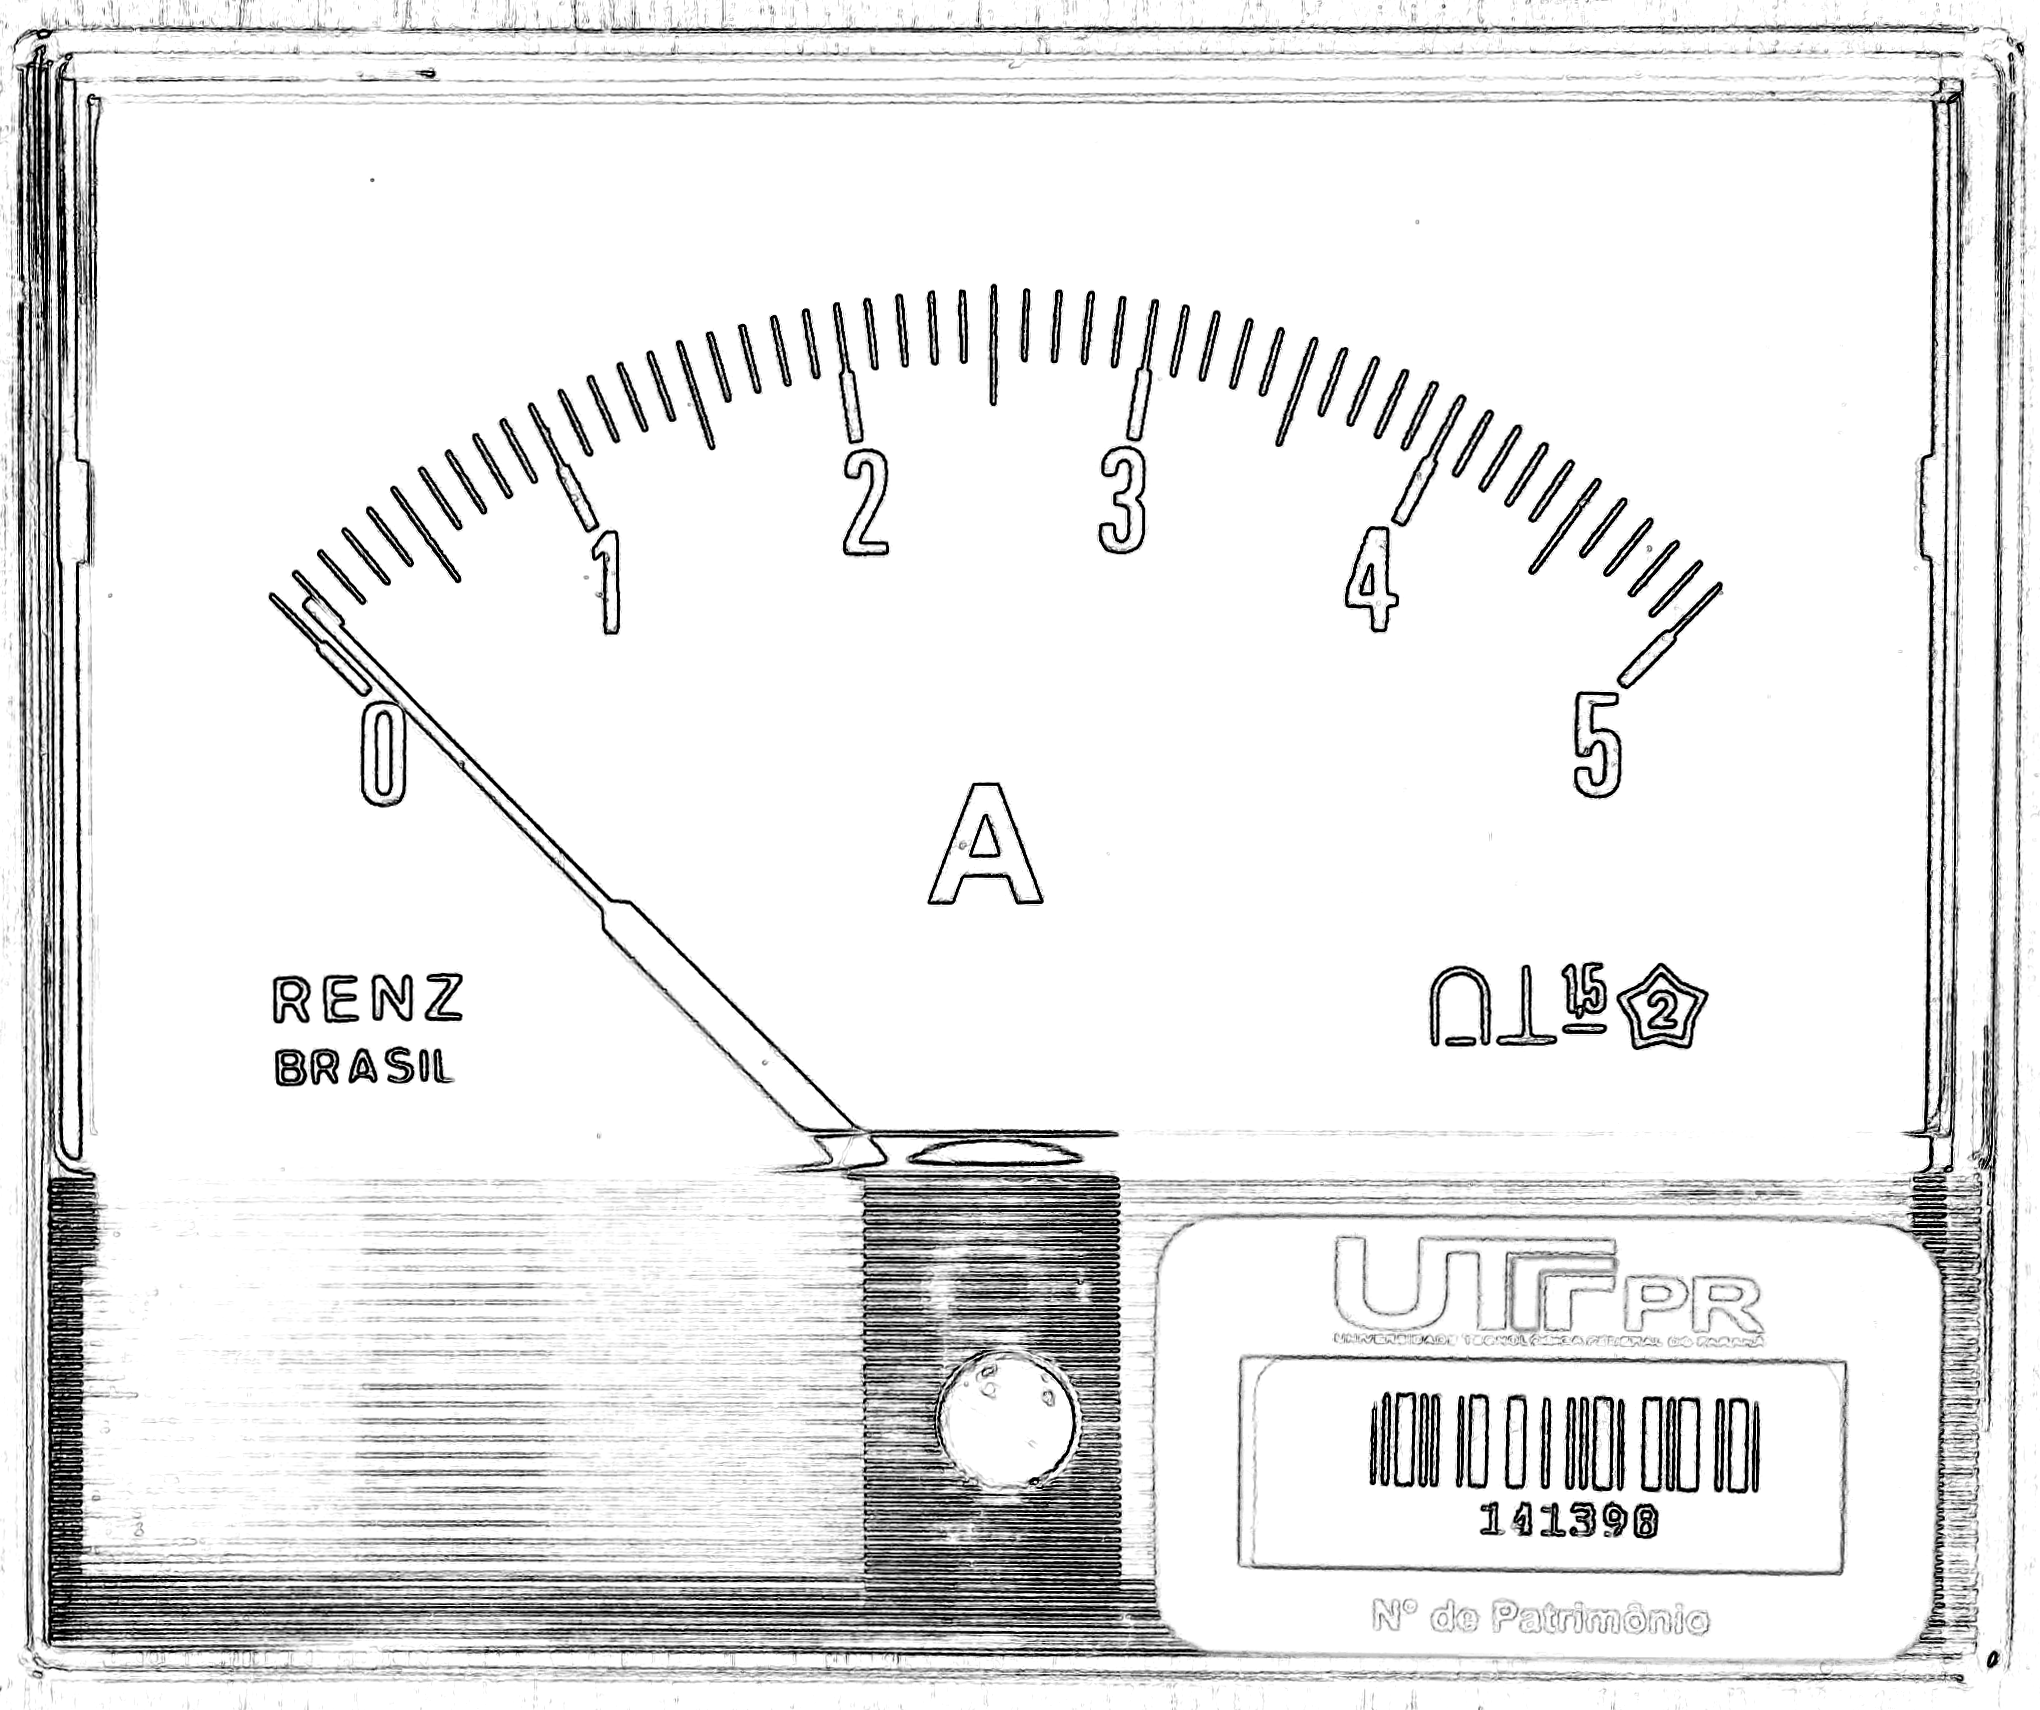
\includegraphics[width=0.97\linewidth]{Ilustrations/EscalaPeqDiv.png}
    \caption{Dois equipamentos capazes de realizar medidas em um intervalo de zero a cinco ampéres. Note que a menor divisão da escala é menor no segundo caso.}
\end{marginfigure}

	\item[Equipamentos digitais ou dotados de escala auxiliar:] Se, por outro lado, o equipamento for digital podemos realizar uma medida como $M = \np[g]{14,2}$, por exemplo. Se utilizássemos um equipamento mais preciso, talvez essa medida pudesse variar entre \np[g]{14,15} até \np[g]{14,25} (incluindo o primeiro valor, porém não incluindo o último) devido a arredondamentos realizados pelo equipamento em virtude do número reduzido de casas decimais. Outra possibilidade é a de que o equipamento simplesmente descarte dígitos menores que décimos de grama, o que permitiria que as medidas variassem entre \np[g]{14,20} e \np[g]{14,29}. Poderíamos escolher para o erro do equipamento o valor de metade da menor divisão da escala abaixo do valor mostrado e de uma divisão acima. Por simplicidade, no entanto, \emph{assumimos que no caso de equipamentos digitais o erro é equivalente à menor divisão da escala tanto acima quanto abaixo do valor indicado}.
	
	Se o equipamento é dotado de uma escala auxiliar, verificamos que ao realizar a leitura em geral percebemos que duas ou três marcar parecem alinhadas com as marcas da escala principal. Se tormarmos a do meio, por exemplo, poderíamos considerar que a medida pode variar dentro do intervalo compreendido pelas marcas à esquerda e à direita. Logo, também adotamos para o erro a menor divisão da escala. Como tanto os equipamentos digitais, quanto os dotados de escala auxiliar possuem erros dados pela mesma regra, equipamentos desses dois tipos são comumente referidos coletivamente como \emph{não-analógicos}.
\end{description}

%%%%%%%%%%%%%%%%%%%%%%%%%%%
\section{Erros propagados}
%%%%%%%%%%%%%%%%%%%%%%%%%%%

Se precisamos calcular a área de uma folha, é mais fácil realizar um cálculo através do produto das medidas de ambos os lados, que comparar com um ``padrão de área''. Se temos um erro nas medidas das laterais, no entanto, deve haver um erro associado à medida da área.

Na Figura~\ref{Fig:ErroArea} mostramos o cálculo da área a partir de duas medidas $\ell_1$ e $\ell_2$. Como cada uma dessas medidas possui um erro associado, denotados por $\delta\ell_1$ e $\delta\ell_2$, respectivamente, devemos calcular os valores máximos e mínimos da área:
%
\begin{marginfigure}[-2cm]
\centering
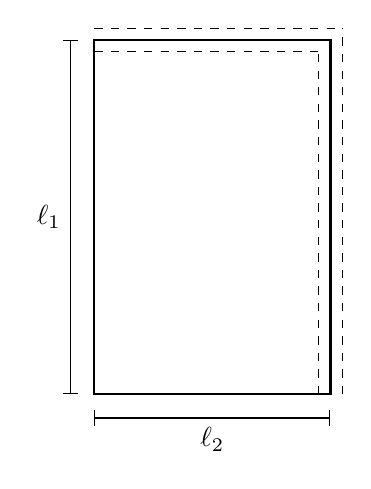
\begin{tikzpicture}[scale=1.5]
	\draw[thick] (0,0) rectangle (2,3);
	\draw[dashed,thin] (1.9,0) -- (1.9,2.9);
	\draw[dashed,thin] (2.1,0) -- (2.1,3.1);
	\draw[dashed,thin] (0,2.9) -- (1.9,2.9);
	\draw[dashed,thin] (0,3.1) -- (2.1,3.1);
	
	\draw[|-|] (-0.2,0) -- node[left]{$\ell_1$} (-0.2,3);
	
	\draw[|-|] (0, -0.2) -- node[below]{$\ell_2$} (2, -0.2);
\end{tikzpicture}
\caption{Erro no cálculo da área de um retângulo.}
\label{Fig:ErroArea}
\end{marginfigure}
%
\begin{align}
	A_{-} &= (\ell_1 - \delta\ell_1)(\ell_2 - \delta\ell_2) \\
	&= \ell_1\ell_2 - (\ell_1 \,\delta\ell_2 + \ell_2\,\delta\ell_1 - \delta\ell_1\,\delta\ell_2) \\
	A_{+} &= (\ell_1 + \delta\ell_1)(\ell_2 + \delta\ell_2) \\
	&= \ell_1\ell_2 + (\ell_1 \,\delta\ell_2 + \ell_2\,\delta\ell_1 + \delta\ell_1\,\delta\ell_2).
\end{align}

\noindent{}Se desprezarmos o produto $\delta\ell_1\,\delta\ell_2$, que deve ser muito pequeno, já que os erros são ---~em geral~--- pequenas frações das medidas, podemos escrever as expressões acima como uma só:
\begin{equation}
	A = \ell_1\ell_2 \pm (\ell_1\,\delta\ell_2+\ell_2\,\delta\ell_1).
\end{equation}
%
Temos então uma expressão para calcular o erro associado à área da folha. 

A expressão acima, não está limitada ao cálculo de uma área, mas serve para qualquer multiplicação de dois números. Veremos adiante que podemos determinar um método geral para a obtenção do erro para qualquer expressão. A partir de tal método, é possível deduzir os resultados abaixo
\begin{subequations}
\begin{align}
	(x\pm\delta x)+(y\pm\delta y) &= (x+y)\pm(\delta x+\delta y) \label{Eq:ErroOpBasica:soma}\\
	(x\pm\delta x)-(y\pm\delta y) &= (x-y)\pm(\delta x + \delta y) \label{Eq:ErroOpBasica:subtracao} \\
	(x\pm\delta x) \cdot (y\pm\delta y) &= (x\cdot y)\pm (|x|\cdot\delta y + |y|\cdot\delta x) \label{Eq:ErroOpBasica:mult} \\
	(x\pm \delta x)\div(y\pm\delta y) &= (x\div y)\pm\frac{|x|\cdot\delta y+|y|\cdot\delta x}{y^2} \label{Eq:ErroOpBasica:div} \\
	(x\pm\delta x)^n &= x^n\pm n \cdot x^{n-1}\cdot\delta x \label{Eq:ErroOpBasica:pot} \\
	\ln(x\pm\delta x) &= \ln x \pm \frac{\delta x}{x} \\
	\log (x\pm\delta x) &= \log x \pm \frac{0,4343\cdot\delta x}{x}.
\end{align}
\end{subequations}
%
É importante observar, no entanto, que apesar de podermos calcular o erro propagado em uma operação complexa como uma sucessão de operações simples ---~como as do conjunto de equações acima~--- em geral esse erro é maior do que aquele que seria obtido se deduzíssemos a expressão para o erro a partir da expressão geral para o erro propagado.

%%%%%%%%%%%%%%%%%%%%%%%%%%%%%%%%%%%%%%%%%%%%%%%%%%
\paragraph{Exemplos de cálculo de erro propagado}
%%%%%%%%%%%%%%%%%%%%%%%%%%%%%%%%%%%%%%%%%%%%%%%%%%

Vamos fazer agora alguns exemplos de operações envolvendo medidas. Para isso, vamos tomar duas medidas $\ell_1$ e $\ell_2$, dadas por
\begin{align}
    \ell_1 &= (\np{13,24} \pm \np{0.05})~\rm{cm} \\
    \ell_2 &= (\np{11.14} \pm \np{0.05})~\rm{cm}.
\end{align}
%
No caso de termos uma soma de tais medidas, temos ---~usando a Equação~\eqref{Eq:ErroOpBasica:soma}~--- 
\begin{align}
    \ell_1 + \ell_2 &= (\np{13,24} \pm \np{0.05})~\rm{cm} + (\np{11.14} \pm \np{0.05})~\rm{cm} \\
    &= ([\np{13,24} + \np{11.14}] \pm [\np{0,05} + \np{0.05}])~\rm{cm} \\
    &= (\np{24,30} \pm \np{0.10})~\rm{cm}.
\end{align}
%
De maneira similar, podemos calcular a diferença entre tais medidas através da Equação~\eqref{Eq:ErroOpBasica:subtracao}:
\begin{align}
    \ell_1 - \ell_2 &= (\np{13,24} \pm \np{0.05})~\rm{cm} - (\np{11.14} \pm \np{0.05})~\rm{cm} \\
    &= ([\np{13,24} - \np{11.14}] \pm [\np{0,05} + \np{0.05}])~\rm{cm} \\
    &= (\np{13,24} \pm \np{0.10})~\rm{cm}.
\end{align}
%
Note que apesar de estarmos realizando uma subtração, os erros são \emph{somados}.

Para o cálculo de um produto, a determinação do erro utilizando a Equação~\eqref{Eq:ErroOpBasica:mult} é um pouco mais elaborada que no caso da soma ou subtração:
\begin{align}
    \ell_1 \ell_2 &= (\np{13,24} \pm \np{0.05})~\rm{cm} \times (\np{11.14} \pm \np{0.05})~\rm{cm} \\
    &= ([\np{13,24} \cdot \np{11.14}] \pm [|\np{13,24}|\cdot\np{0.05} + |\np{11.14}|\cdot\np{0.05}])~\rm{cm}^2 \\
    &= (\np{147,4936} \pm \np{1,219})~\rm{cm}^2 \\
    &= (\np{147,5} \pm \np{1,2})~\rm{cm}^2.
\end{align}
%
Veja que no cálculo acima realizamos todas as operações com toda a precisão disponível ---~isto é, utilizamos todos os dígitos da calculadora~---, mas como último passo descartamos os dígitos cuja ordem de grandeza é menor que a do último algarismo significativo. Esse procedimento deve ser adotado em todos os cálculos envolvendo medidas.

O cálculo do erro na operação de divisão através da Equação~\eqref{Eq:ErroOpBasica:div} é similar ao caso da multiplicação, porém envolve um passo a mais devido à divisão do erro pelo denominador:
\begin{align}
    \ell_1 \div \ell_2 &= (\np{13,24} \pm \np{0.05})~\rm{cm} \div (\np{11.14} \pm \np{0.05})~\rm{cm} \\
    &= \left([\np{13,24} \div \np{11.14}] \pm \left[\frac{|\np{13,24}|\cdot\np{0.05} + |\np{11.14}|\cdot\np{0.05}}{\np{11.14}^2}\right]\right) \\
    &= (\np{1,188509874} \pm \np{0,009822755}) \\
    &= (\np{1,189} \pm \np{0,010}).
\end{align}

Para a potencia, temos no caso geral a Expressão~\eqref{Eq:ErroOpBasica:pot}. Tal equação deve ser particularizada para a potência em questão:
\begin{align}
    \ell_1^2 &= [(\np{13,24} \pm \np{0.05})~\rm{cm}]^2 \\
    &= (\np{13,24}^2 \pm [2 \cdot \np{13,24}^{(2-1)} \cdot \np{0.05}])]~\rm{cm}^2 \\
    &= (\np{175,2976} \pm \np{1,324})~\rm{cm}^2 \\
    &= (\np{175,3} \pm \np{1,3})~\rm{cm}^2.
\end{align}
%
Também podemos utilizar a Expressão~\eqref{Eq:ErroOpBasica:pot} para o cálculo de potências negativas. Para o caso $n = -1$ em especial, temos
\begin{align}
    \ell_1^{-1} &= [(\np{13,24} \pm \np{0.05})~\rm{cm}]^{(-1)} \\
    &= (\np{13,24}^{(-1)} \pm [(-1) \cdot \np{13,24}^{((-1)-1)} \cdot \np{0.05}])]~\rm{cm}^{-1} \\
    &= (\np{0,075528701} \pm [\np{13,24}^{(-2)} \cdot \np{0.05}])]~\rm{cm}^{-1} \\
    &= (\np{0,075528701} \pm \np{0,000285229})~\rm{cm}^{-1} \\
    &= (\np{0,07553} \pm \np{0,0003})~\rm{cm}^{-1} \\
    &= (\np{7,553} \pm \np{0,03})\cdot 10^{-2}~\rm{cm}^{-1}.
\end{align}

As operações exemplificadas acima são as que aparecem com maior frequência em cálculos. Muitas vezes, no entanto, será necessário aplicar mais que uma fórmula. Se, por exemplo, precisamos determinar o resultado de uma expressão do tipo
\begin{equation}
    R = \frac{\ell_1 (\ell_2 - \ell_3)}{\ell_4},
\end{equation}
%
devemos separar o cálculo em etapas, calculando o erro em cada uma delas:
\begin{itemize}
    \item Primeiro calculamos a diferença $d = \ell_2 - \ell_3$;
    \item Após isso, calculamos o produto $p = \ell_1 \cdot d$;
    \item Finalmente, determinamos razão $R = p / \ell_4$.
\end{itemize}

%%%%%%%%%%%%%%%%%%%%%%%%%%%%%%%%%%%%%%%%%%
\subsection{Constantes e erros propagados}
%%%%%%%%%%%%%%%%%%%%%%%%%%%%%%%%%%%%%%%%%%

No caso de termos operações envolvendo constantes como $\pi$, ou qualquer outro valor conhecido absolutamente (como 2, 3, 4, etc.) ---~isto é, que não são medidas~---, podemos simplesmente efetuar a operação com a constante e o erro da mesma forma que com a medida. Por exemplo
\begin{align}
     r &= (\numprint{4,0} \pm \numprint{0,5})\textrm{~mm} \\
     p &= 2\pi r \\
     &= 2\pi(\numprint{4,0} \pm \numprint{0,5})\textrm{~mm} \\
     &= (2\pi\,\numprint{4,0} \pm 2\pi\,\numprint{0,5})\textrm{~mm} \\
     &= (25 \pm 3)~\textrm{~mm}
\end{align}
%
sempre respeitando o número de algarismos significativos e os critérios de arredondamento.

%%%%%%%%%%%%%%%%%%%%%%%%%%%%%%%%%%%%%%%%%%%%%%
\section{Erros e algarismos significativos}
%%%%%%%%%%%%%%%%%%%%%%%%%%%%%%%%%%%%%%%%%%%%%%

Verificamos que as medidas fornecidas por instrumentos são expressas por um conjunto de algarismos significativos e que algarismos além deles são mera especulação. Também utilizamos regras gerais para determinar o número de algarismos significativos de uma medida indireta com base no número de algarismos significativos das medidas diretas. Agora que conhecemos o erro, podemos entender a origem dos algarismos significativos de uma maneira simples: eles são os algarismos cuja ordem de grandeza é maior ou igual àquela do erro. %\comment{Existem casos em que o erro propagado pode ser maior ou menor que o último significativo, o que fazer nesse caso?}

Para verificar como funciona esse processo, vejamos o seguinte conjunto de medidas:
\begin{align}
	v_0 &= (\numprint{10,3456} \pm \numprint{0,01})~\textrm{m}/\textrm{s} \label{medidas_v_start}\\
	a &= (\numprint{2,0658} \pm \numprint{0,05})~\textrm{m}/\textrm{s}^2 \\
	t &= (\numprint{3,000} \pm \numprint{0,001})~\textrm{s} \label{medidas_v_end}.
\end{align}
%
Utilizando essas informações e as fórmulas para o erro propagado, obtemos ---~utilizando a relação $v = v_0 + at$~--- o seguinte resultado:
\begin{equation}
	v = (\numprint{16,543} \pm \numprint{0,1620658})~\textrm{m}/\textrm{s}.
\end{equation}
%
O erro é sempre expresso com um ou dois algarismos significativos\footnote{Lembre-se que utilizamos dois se o primeiro algarismo significativo do erro, isto é, o primeiro dígito diferente de zero, for 1; nos demais casos utilizamos somente um algarismo significativo.}. Nesse caso, o erro da medida acima pode ser expresso como $\delta v = \np[m/s]{0,16}$. Vemos também que a medida tem algarismos cuja ordem de grandeza é menor que o erro e são, portanto, sem significado. Podemos reduzir nossa medida para a velocidade a
\begin{equation}\label{ResultadoAlgSigErro}
	v = (\numprint{16,54} \pm \numprint{0,16})~\textrm{m}/\textrm{s}.
\end{equation}

Analisando o erro das medidas mostradas nas Equações~\eqref{medidas_v_start} a~\eqref{medidas_v_end}, percebemos que existem vários algarismos sem significado. Retirando-os, obtemos
\begin{align}
	v_0 &= (\numprint{10,35} \pm \numprint{0,01})~\textrm{m}/\textrm{s} \\
	a &= (\numprint{2,07} \pm \numprint{0,05})~\textrm{m}/\textrm{s}^2 \\
	t &= (\numprint{3,000} \pm \numprint{0,001})~\textrm{s}.
\end{align}
%
Verificamos agora que a medida para a aceleração $a$ tem somente três algarismos significativos. Segundo a regra sobre o número de algarismos significativos para o resuldado de uma multiplicação, devemos manter então somente três algarismos. Ao somarmos com o valor de $v_0$, a regra nos diz para mantermos duas casas após a vírgula. De fato, isto nos dá um resultado que coincide com aquele obtido através da análise do erro propagado (Equação~\eqref{ResultadoAlgSigErro}).

%\comment{Em alguns casos o erro fica menor do que o último algarismo duvidoso (pelo menos observei isso em alguns cálculos hipotéticos). E aí? Existem casos em que o erro fique maior, forçando a descartar algarismos?}

%%%%%%%%%%%%%%%%%%%%%%%%%%%%%%%%%%%%%%%%%%%%%
\section{Incerteza fracional e percentual}
%%%%%%%%%%%%%%%%%%%%%%%%%%%%%%%%%%%%%%%%%%%%%

Se realizamos uma medição com um instrumento e obtemos $\ell_1 = (\numprint{15,3} \pm \numprint{0,5})~\textrm{cm}$, o erro é de aproximadamente \numprint{3,3}\%. Se realizarmos outra medição com o mesmo instrumento e obtivermos $\ell_2 = (\numprint{3,4} \pm \numprint{0,5})~\textrm{cm}$, teremos um erro de aproximadamente \numprint{14,7}\%. Claramente no segundo caso temos uma medida mais incerta que no primeiro, o que acarretará em consequências para o cálculo de medidas indiretas.

Para calcularmos o erro como uma fração da medida, basta o dividirmos pelo valor da medida:
\begin{equation}
	E_f = \frac{\delta x}{x}.
\end{equation}
%
Como $x$ e $\delta x$ possuem a mesma unidade, o erro fracional é adimensional. O erro percentual pode ser calculado multiplicando-se o erro fracional por 100:
\begin{equation}
	E_\% = 100 \cdot E_f.
\end{equation}

É comum encontrar dispositivos eletrônicos cujo erro é dado como um número percentual. Por exemplo, podemos ter um resistor cuja resistência $R$ é de $500~\Omega$, com erro de $5~\%$. Isso significa que a medida da resistência é $R = (500 \pm 25)~\Omega$, ou melhor, $R = (5,0 \pm 0,3)\cdot 10^2~\Omega$. 

Outro uso comum do erro percentual é ao se declarar a precisão de um instrumento de medida. Se um voltímetro declara sua precisão como $1~\%$, isso significa que em uma medida $V_1 = \numprint[V]{13,45}$ temos um erro  $\delta V_1 = \numprint[V]{0,13}$. Já em uma medida $V_2 = \numprint[V]{156,35}$, temos um erro $\delta V_2 = \numprint[V]{1,6}$. Temos, portanto, um caso em que o erro da medida ---~também chamado de \emph{erro absoluto}~--- varia, mas o erro percentual é constante, indicando que o instrumento é igualmente adequado (ou inadequado, dependendo de sua necessidade de precisão) para uma ampla faixa de valores de medida.

Os erros fracional e percentual nos indicam que sempre que desejarmos conhecer uma medida calculada a partir de outras, devemos procurar utilizar medidas diretas com um grande número de algarismos significativos, de forma a minimizar o erro percentual. Por exemplo, se calcularmos o valor da aceleração da gravidade através de
\begin{equation}
	g = \frac{2\Delta x}{t^2},
\end{equation}
%
a partir das medidas 
\begin{align}
	t_1 &= (\numprint{0,15} \pm \numprint{0,01})~\textrm{s} \\
	\Delta x_1 &= (\numprint{0,11} \pm \numprint{0,02})~\textrm{m}
\end{align}
%
e
\begin{align}
	t_2 &= (\numprint{1,32} \pm \numprint{0,01})~\textrm{s} \\
	\Delta x_2 &= (\numprint{8,54} \pm \numprint{0,02})~\textrm{m},
\end{align}
%
obteremos os valores
\begin{align}
	g_1 &= (\numprint{9,8} \pm 2)~\textrm{m}/\textrm{s}^2 \\
	g_2 &= (\numprint{9,80} \pm \numprint{0,1})~\textrm{m}/\textrm{s}^2.
\end{align}
%
Claramente as medidas diretas têm o mesmo erro absoluto, no entanto erros fracionais/percentuais diferentes. Isso se reflete na incerteza da medida indireta, onde no segundo caso obtemos um erro muito menor, devido ao menor erro fracional/percentual.

%%%%%%%%%%%%%%%%%%%%%%%%%%%%%%%%%%%%%%%%%%%%%%%%%%%%%%%%%%%%%%%%
\subsection{Erro percentual em relação a um valor de referência}
%%%%%%%%%%%%%%%%%%%%%%%%%%%%%%%%%%%%%%%%%%%%%%%%%%%%%%%%%%%%%%%%

Em experiências didáticas, é muito comum que estejamos interessados em determinar o valor de uma constante física cujo valor já é conhecido experimentalmente com grande precisão. Nesses casos, é interessante obter um valor percentual de diferença entre o valor obtido e o valor de referência. Tal valor também é conhecido como erro percentual, e pode ser calculado através da expressão
\begin{equation}
    E_\% = \left|\frac{x - x_{\rm{ref}}}{x_{\rm{ref}}}\right| \cdot 100,
\end{equation}
%
onde $x$ representa o valor que obtemos experimentalmente e $x_{\rm{ref}}$ representa o valor de referência.

%%%%%%%%%%%%%%%%%%%%%%%%%%%%%%%%%%%%%%%%%%%%%%%%%%%%%%%%%%%%%
\section{Expressão geral para o cálculo do erro propagado}
%%%%%%%%%%%%%%%%%%%%%%%%%%%%%%%%%%%%%%%%%%%%%%%%%%%%%%%%%%%%%
%\comment{Ver aqui se tem algum problema, tinha uns errinhos e tinha que substituir uns $d$ por $\delta$.}
Apesar de termos conseguido calcular o erro propagado de uma maneira relativamente simples para o caso do produto de duas medidas, precisamos de um método mais robusto, que possa sem aplicado a \emph{qualquer tipo de função}. Se tivermos uma medida $q$, dada por $q=f(x,y,z,\dots,\xi,\dots)$, onde $x$, $y$, $z$, \dots, $\xi$, \dots representam medidas diretas através das quais calculamos a medida indireta $q$, podemos calcular uma variação em $q$ em relação a uma variação em uma das medidas ---~na medida $\xi$, por exemplo~--- através de uma derivada:
\begin{equation}
	\frac{dq}{d\xi} = \frac{df(x,y,z,\dots,\xi,\dots)}{d\xi}.
\end{equation}
%
Podemos então escrever a variação $dq$ como 
\begin{equation}
	dq = \left(\frac{df(x,y,z,\dots,\xi,\dots)}{d\xi}\right)d\xi.
\end{equation}
%
Assumindo que as variáveis $x$, $y$, $z$, \dots, $\xi$ são todas independentes, podemos escrever a expressão acima como
\begin{equation}
    dq = \left(\frac{\partial f(x,y,z,\dots,\xi)}{\partial \xi}\right)d\xi.
\end{equation}
%
Agora podemos identificar as variações $d\xi$ e $dq$ na expressão acima com próprios erros nas medidas. Logo, a contribuição para o erro em $q$ devido ao erro $\delta\xi$ é dada por
\begin{equation}
    \delta q = \left(\frac{\partial f(x,y,z,\dots,\xi)}{\partial \xi}\right)\delta\xi.
\end{equation}
%
Cada uma das medidas dá origem a um termo análogo à expressão acima. Somando todas essas contribuições, obtemos
\begin{equation}\label{Eq:ErroGeral}
	\delta q = \left|\frac{\partial f}{\partial x}\right| \delta x + \left|\frac{\partial f}{\partial y}\right| \delta y + \left|\frac{\partial f}{\partial z}\right| \delta z + \dots + \left|\frac{\partial f}{\partial \xi}\right| \delta\xi,
\end{equation}
%
onde tomamos o valor absoluto da derivada parcial para eliminar possíveis ``compensações'' devido a sinais diferentes para cada termo.

A partir da equação acima, podemos calcular o erro para qualquer função que nos dê uma medida indireta. Se, por exemplo, considerarmos a área de um retângulo
\begin{equation}
    A = f(\ell_1,\ell_2)=\ell_1\ell_2,
\end{equation}
%
temos:
\begin{align}
	\delta A &= \left|\frac{\partial(\ell_1\ell_2)}{\partial \ell_1}\right|\delta \ell_1 + \left|\frac{\partial (\ell_1\ell_2)}{\partial \ell_2}\right|\delta \ell_2 \\
	&= |\ell_2|\delta \ell_1 + |\ell_1|\delta \ell2,
\end{align}
%
que é exatamente a expressão que encontramos quando analisamos os valores máximo e mínimo para a área do retângulo. 

%%%%%%%%%%%%%%%%%%%%%%%%%%%%%%%%%%%%%%%%%
%\section{Representando erros em gráficos}
%%%%%%%%%%%%%%%%%%%%%%%%%%%%%%%%%%%%%%%%%

%\comment{Falar e dar exemplos de barras de erro (simétricas, assimétricas)}



